% Options for packages loaded elsewhere
\PassOptionsToPackage{unicode}{hyperref}
\PassOptionsToPackage{hyphens}{url}
%
\documentclass[
  ignorenonframetext,
]{beamer}
\usepackage{pgfpages}
\setbeamertemplate{caption}[numbered]
\setbeamertemplate{caption label separator}{: }
\setbeamercolor{caption name}{fg=normal text.fg}
\beamertemplatenavigationsymbolsempty
% Prevent slide breaks in the middle of a paragraph
\widowpenalties 1 10000
\raggedbottom
\setbeamertemplate{part page}{
  \centering
  \begin{beamercolorbox}[sep=16pt,center]{part title}
    \usebeamerfont{part title}\insertpart\par
  \end{beamercolorbox}
}
\setbeamertemplate{section page}{
  \centering
  \begin{beamercolorbox}[sep=12pt,center]{part title}
    \usebeamerfont{section title}\insertsection\par
  \end{beamercolorbox}
}
\setbeamertemplate{subsection page}{
  \centering
  \begin{beamercolorbox}[sep=8pt,center]{part title}
    \usebeamerfont{subsection title}\insertsubsection\par
  \end{beamercolorbox}
}
\AtBeginPart{
  \frame{\partpage}
}
\AtBeginSection{
  \ifbibliography
  \else
    \frame{\sectionpage}
  \fi
}
\AtBeginSubsection{
  \frame{\subsectionpage}
}
\usepackage{lmodern}
\usepackage{amssymb,amsmath}
\usepackage{ifxetex,ifluatex}
\ifnum 0\ifxetex 1\fi\ifluatex 1\fi=0 % if pdftex
  \usepackage[T1]{fontenc}
  \usepackage[utf8]{inputenc}
  \usepackage{textcomp} % provide euro and other symbols
\else % if luatex or xetex
  \usepackage{unicode-math}
  \defaultfontfeatures{Scale=MatchLowercase}
  \defaultfontfeatures[\rmfamily]{Ligatures=TeX,Scale=1}
\fi
\usecolortheme{dolphin}
% Use upquote if available, for straight quotes in verbatim environments
\IfFileExists{upquote.sty}{\usepackage{upquote}}{}
\IfFileExists{microtype.sty}{% use microtype if available
  \usepackage[]{microtype}
  \UseMicrotypeSet[protrusion]{basicmath} % disable protrusion for tt fonts
}{}
\makeatletter
\@ifundefined{KOMAClassName}{% if non-KOMA class
  \IfFileExists{parskip.sty}{%
    \usepackage{parskip}
  }{% else
    \setlength{\parindent}{0pt}
    \setlength{\parskip}{6pt plus 2pt minus 1pt}}
}{% if KOMA class
  \KOMAoptions{parskip=half}}
\makeatother
\usepackage{xcolor}
\IfFileExists{xurl.sty}{\usepackage{xurl}}{} % add URL line breaks if available
\IfFileExists{bookmark.sty}{\usepackage{bookmark}}{\usepackage{hyperref}}
\hypersetup{
  pdftitle={Title in Progress},
  hidelinks,
  pdfcreator={LaTeX via pandoc}}
\urlstyle{same} % disable monospaced font for URLs
\newif\ifbibliography
\usepackage{graphicx,grffile}
\makeatletter
\def\maxwidth{\ifdim\Gin@nat@width>\linewidth\linewidth\else\Gin@nat@width\fi}
\def\maxheight{\ifdim\Gin@nat@height>\textheight\textheight\else\Gin@nat@height\fi}
\makeatother
% Scale images if necessary, so that they will not overflow the page
% margins by default, and it is still possible to overwrite the defaults
% using explicit options in \includegraphics[width, height, ...]{}
\setkeys{Gin}{width=\maxwidth,height=\maxheight,keepaspectratio}
% Set default figure placement to htbp
\makeatletter
\def\fps@figure{htbp}
\makeatother
\setlength{\emergencystretch}{3em} % prevent overfull lines
\providecommand{\tightlist}{%
  \setlength{\itemsep}{0pt}\setlength{\parskip}{0pt}}
\setcounter{secnumdepth}{-\maxdimen} % remove section numbering

\title{Title in Progress}
\author{Amy Pitts, Hun Lee, Jimmy Kelliher,\\
Tucker Morgan, and Waveley Qiu}
\date{2022-02-21}

\begin{document}
\frame{\titlepage}

\begin{frame}{Motivation}
\protect\hypertarget{motivation}{}

\begin{itemize}[<+->]
\tightlist
\item
  Identifying the effect of a treatment or intervention is one of the
  most fundamental tasks we encounter as biostatisticians\ldots{}
\end{itemize}

\begin{itemize}[<+->]
\tightlist
\item
  \ldots{} but outside of a randomized control trial (RCT), confounding
  variables can bias our estimates of treatment effects.
\end{itemize}

\begin{itemize}[<+->]
\tightlist
\item
  Propensity score matching (PSM) is a tool that can help us mitigate
  the effects of confounders\ldots{}
\end{itemize}

\begin{itemize}[<+->]
\tightlist
\item
  \ldots{} but there is no consensus on the best way to estimate
  standard errors when using the PSM algorithm.
\end{itemize}

\begin{itemize}[<+->]
\tightlist
\item
  How can we assess which procedures reliably estimate standard errors?
\end{itemize}

\end{frame}

\begin{frame}{Motivation}
\protect\hypertarget{motivation-1}{}

\begin{center}
  A simulation study!
\end{center}

\end{frame}

\begin{frame}{A Quick Foray into Confounding}
\protect\hypertarget{a-quick-foray-into-confounding}{}

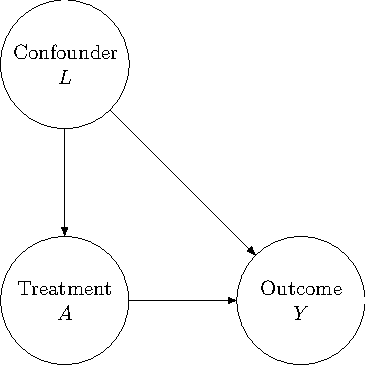
\includegraphics{pres_draft_jimmy_files/figure-beamer/unnamed-chunk-1-1.pdf}

\end{frame}

\begin{frame}{Taking a Step Back, What is Propensity Score Matching?}
\protect\hypertarget{taking-a-step-back-what-is-propensity-score-matching}{}

\begin{itemize}[<+->]
\tightlist
\item
  A \emph{propensity score} is the probability that an individual
  receives a treatment \(A\); that is, \(P(A = 1)\). In an RCT,
  treatments are randomized, and hence outcomes \(Y\) are independent of
  treatment \(A\).
\end{itemize}

\end{frame}

\begin{frame}{Enter the Bootstrap}
\protect\hypertarget{enter-the-bootstrap}{}

\begin{itemize}[<+->]
\tightlist
\item
  Bootstrapping is one of the most common procedures for estimating
  standard errors.
\end{itemize}

\begin{itemize}[<+->]
\tightlist
\item
  The PSM algorithm intakes an unmatched dataset and outputs a matched
  one.
\end{itemize}

\begin{itemize}[<+->]
\tightlist
\item
  When do we execute the bootstrap - before the match or after it?
\end{itemize}

\begin{itemize}[<+->]
\tightlist
\item
  Let's try both!
\end{itemize}

\end{frame}

\begin{frame}{Roadmap of the Simulation Study}
\protect\hypertarget{roadmap-of-the-simulation-study}{}

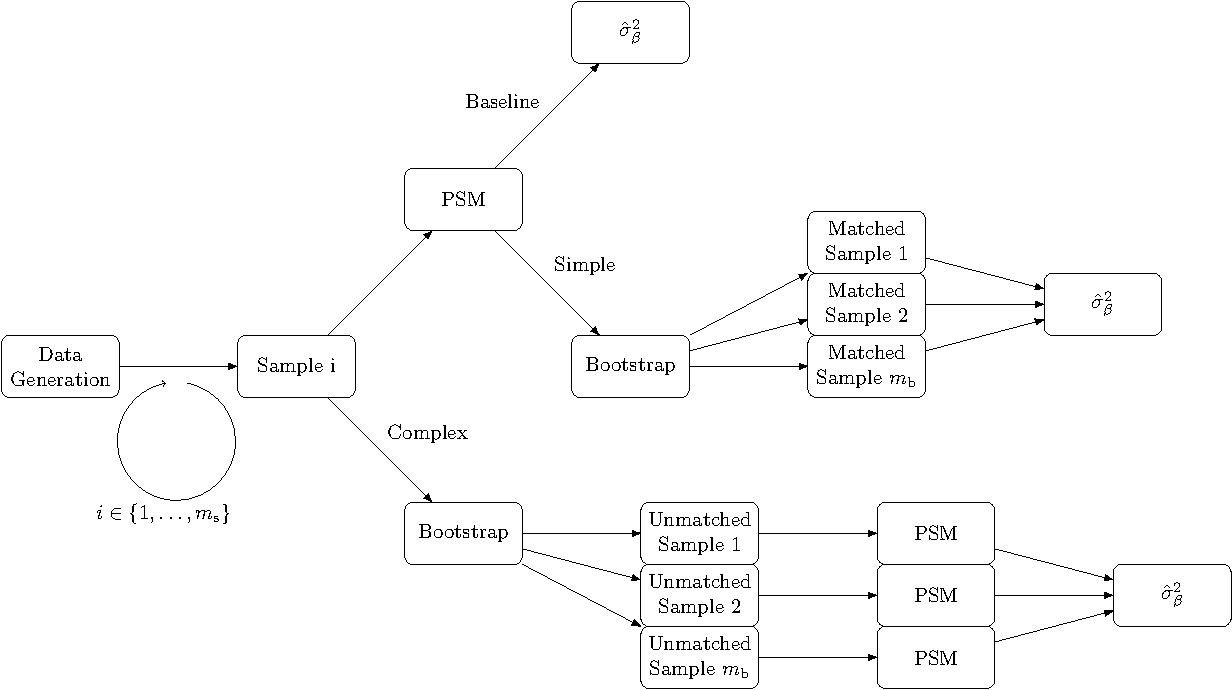
\includegraphics{pres_draft_jimmy_files/figure-beamer/unnamed-chunk-2-1.pdf}

\end{frame}

\begin{frame}{Data Generation}
\protect\hypertarget{data-generation}{}

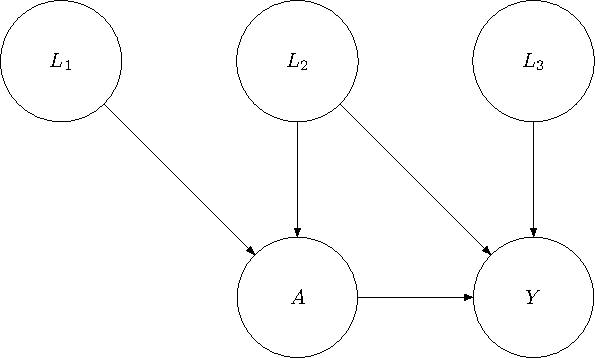
\includegraphics{pres_draft_jimmy_files/figure-beamer/unnamed-chunk-3-1.pdf}

\end{frame}

\begin{frame}{Data Generation - Continuous Outcome}
\protect\hypertarget{data-generation---continuous-outcome}{}

For each individual \(i \in \{ 1, \ldots, n \}\), we consider covariates
\(L_{1i}, L_{2i}, L_{3i} \sim N(0, 1)\). Treatments are distributed
according to law \(A_i \sim B(\pi_i)\), where \(\pi_i\) - the true
propensity to be treated - is subject to the data-generating process \[
    \log \left( \frac{\pi_i}{1 - \pi_i} \right)
    = \alpha_0 + \alpha_1 L_{1i} + \alpha_2 L_{2i}.
  \] Given this, we further define the data-generating process of our
continuous outcome via
\[ Y_i = \beta_1 A_i + \beta_2 L_{2i} + \beta_3 L_{3i} + \varepsilon_i, \]
where \(\varepsilon_i\) denotes random error. Because \(L_{2i}\) effects
both \(A_i\) and \(Y_i\), it acts as a confounder in estimating the
treatment effect.

\end{frame}

\begin{frame}{Data Generation - Binary Outcome}
\protect\hypertarget{data-generation---binary-outcome}{}

For each individual \(i \in \{ 1, \ldots, n \}\), we consider covariates
\(L_{1i}, L_{2i}, L_{3i} \sim N(0, 1)\). Treatments are distributed
according to law \(A_i \sim B(\pi_i)\), where \(\pi_i\) - the true
propensity to be treated - is subject to the data-generating process \[
    \log \left( \frac{\pi_i}{1 - \pi_i} \right)
    = \alpha_0 + \alpha_1 L_{1i} + \alpha_2 L_{2i}.
  \] Given this, we further define the data-generating process of our
binary outcome via \(Y_i \sim B(\tau_i)\) where \[
    \log \left( \frac{\tau_i}{1 - \tau_i} \right)
    = \beta_1 A_i + \beta_2 L_{2i} + \beta_3 L_{3i}.
  \] Observe that we have omitted a random error term, as realizations
of \(Y_i\) are innately subject to noise.

\end{frame}

\begin{frame}{Parameters of Interest}
\protect\hypertarget{parameters-of-interest}{}

\begin{itemize}
\tightlist
\item
  The sample size of each dataset
  \(n_{\text{sample}} \in \{ 100, 1000 \}\)
\item
  The population proportion of treated individuals
  \(\pi \in \{ 0.113, 0.216, 0.313 \}\)
\item
  The true average treatment effect \(\beta_1 \in \{0.15, 0.30 \}\)
\end{itemize}

\emph{Other Parameters}

\begin{itemize}
\tightlist
\item
  The number of datasets \(m_{\text{sample}} = 100\)
\item
  The number of bootstrap re-sample \(m_{\text{boot}} = 500\)
\item
  The sample size of bootstrap re-samples
  \(n_{\text{simple}} = n_{\text{complex}} = n_{\text{sample}}\times \pi\)
\item
  Strength of Covariate Correlation on Treatment Status
  \(\alpha_1, \alpha_2\) (continuous data (1,2), binary data
  (\(\log(1.25), \log(1.75)\)) )
\item
  Strength of Covariate Correlation on Outcome Variable
  \(\beta_2, \beta_3\) (continuous data (2,1), binary data
  (\(\log(1.75), \log(1.25)\)) )
\end{itemize}

\end{frame}

\begin{frame}{Measures of Interest}
\protect\hypertarget{measures-of-interest}{}

\begin{itemize}
\tightlist
\item
  \textbf{Coverage Rate:} Looks at the rate of the true avergae
  treatment effect falling in the 95\% confidence intervals.
  \(\hat{\text{ATE}} \pm 1.96\times \text{SE}\)
\item
  \textbf{Standard Error:} the variability of the average estimate.
\end{itemize}

\emph{Other Measures}

\begin{itemize}
\tightlist
\item
  \textbf{Bias:} This is mean of the average estimate subtract the true
  ATE
\item
  \textbf{95\% Confidence Intervals:}
\end{itemize}

\end{frame}

\begin{frame}{Results}
\protect\hypertarget{results}{}

\includegraphics{pres_draft_jimmy_files/figure-beamer/loading in binary coverage plot-1.pdf}

\end{frame}

\begin{frame}[fragile]{Results}
\protect\hypertarget{results-1}{}

\begin{verbatim}
## Warning: Removed 1 rows containing missing values (geom_point).
\end{verbatim}

\includegraphics{pres_draft_jimmy_files/figure-beamer/binary standard error plot-1.pdf}

\end{frame}

\begin{frame}{Results}
\protect\hypertarget{results-2}{}

\includegraphics{pres_draft_jimmy_files/figure-beamer/continuous coverage plot-1.pdf}

\end{frame}

\begin{frame}{Results}
\protect\hypertarget{results-3}{}

\includegraphics{pres_draft_jimmy_files/figure-beamer/continous standard error plot-1.pdf}

\end{frame}

\begin{frame}{Summary of Results}
\protect\hypertarget{summary-of-results}{}

\end{frame}

\begin{frame}{Limitations}
\protect\hypertarget{limitations}{}

\begin{itemize}[<+->]
\tightlist
\item
  Sample size / treatment (or exposure) prevalence
\end{itemize}

\begin{itemize}[<+->]
\tightlist
\item
  Small number of initial samples, limited in detecting differences in
  coverage rate
\end{itemize}

\begin{itemize}[<+->]
\item
\end{itemize}

\begin{itemize}[<+->]
\item
\end{itemize}

\end{frame}

\begin{frame}{Future Work}
\protect\hypertarget{future-work}{}

\begin{itemize}[<+->]
\tightlist
\item
  Larger number of initial samples, narrower coverage window
\end{itemize}

\begin{itemize}[<+->]
\tightlist
\item
  Increased sample size, changes in bootstrap performance?
\end{itemize}

\begin{itemize}[<+->]
\tightlist
\item
  Changes in treatment propensity model
\end{itemize}

\begin{itemize}[<+->]
\tightlist
\item
  Non-normal distributions of covariates
\end{itemize}

\end{frame}

\end{document}
